% Options for packages loaded elsewhere
\PassOptionsToPackage{unicode}{hyperref}
\PassOptionsToPackage{hyphens}{url}
%
\documentclass[
]{article}
\usepackage{lmodern}
\usepackage{amssymb,amsmath}
\usepackage{ifxetex,ifluatex}
\ifnum 0\ifxetex 1\fi\ifluatex 1\fi=0 % if pdftex
  \usepackage[T1]{fontenc}
  \usepackage[utf8]{inputenc}
  \usepackage{textcomp} % provide euro and other symbols
\else % if luatex or xetex
  \usepackage{unicode-math}
  \defaultfontfeatures{Scale=MatchLowercase}
  \defaultfontfeatures[\rmfamily]{Ligatures=TeX,Scale=1}
\fi
% Use upquote if available, for straight quotes in verbatim environments
\IfFileExists{upquote.sty}{\usepackage{upquote}}{}
\IfFileExists{microtype.sty}{% use microtype if available
  \usepackage[]{microtype}
  \UseMicrotypeSet[protrusion]{basicmath} % disable protrusion for tt fonts
}{}
\makeatletter
\@ifundefined{KOMAClassName}{% if non-KOMA class
  \IfFileExists{parskip.sty}{%
    \usepackage{parskip}
  }{% else
    \setlength{\parindent}{0pt}
    \setlength{\parskip}{6pt plus 2pt minus 1pt}}
}{% if KOMA class
  \KOMAoptions{parskip=half}}
\makeatother
\usepackage{xcolor}
\IfFileExists{xurl.sty}{\usepackage{xurl}}{} % add URL line breaks if available
\IfFileExists{bookmark.sty}{\usepackage{bookmark}}{\usepackage{hyperref}}
\hypersetup{
  pdftitle={Project Report},
  pdfauthor={Caroline Andy, Vasili Fokaidis, Stella Li, Tessa Senders, Lily Wang},
  hidelinks,
  pdfcreator={LaTeX via pandoc}}
\urlstyle{same} % disable monospaced font for URLs
\usepackage[margin=1in]{geometry}
\usepackage{longtable,booktabs}
% Correct order of tables after \paragraph or \subparagraph
\usepackage{etoolbox}
\makeatletter
\patchcmd\longtable{\par}{\if@noskipsec\mbox{}\fi\par}{}{}
\makeatother
% Allow footnotes in longtable head/foot
\IfFileExists{footnotehyper.sty}{\usepackage{footnotehyper}}{\usepackage{footnote}}
\makesavenoteenv{longtable}
\usepackage{graphicx,grffile}
\makeatletter
\def\maxwidth{\ifdim\Gin@nat@width>\linewidth\linewidth\else\Gin@nat@width\fi}
\def\maxheight{\ifdim\Gin@nat@height>\textheight\textheight\else\Gin@nat@height\fi}
\makeatother
% Scale images if necessary, so that they will not overflow the page
% margins by default, and it is still possible to overwrite the defaults
% using explicit options in \includegraphics[width, height, ...]{}
\setkeys{Gin}{width=\maxwidth,height=\maxheight,keepaspectratio}
% Set default figure placement to htbp
\makeatletter
\def\fps@figure{htbp}
\makeatother
\setlength{\emergencystretch}{3em} % prevent overfull lines
\providecommand{\tightlist}{%
  \setlength{\itemsep}{0pt}\setlength{\parskip}{0pt}}
\setcounter{secnumdepth}{-\maxdimen} % remove section numbering

\title{Project Report}
\author{Caroline Andy, Vasili Fokaidis, Stella Li, Tessa Senders, Lily Wang}
\date{12/11/2020}

\begin{document}
\maketitle

\hypertarget{abstract}{%
\subsection{Abstract}\label{abstract}}

\textbf{Background:}~ Hate crimes are currently the highest priority of
the FBI's civil rights program. Existing research suggests that various
community-level socioeconomic factors, such as income inequality, are
associated with hate crime rate.

\textbf{Objectives:}\\
We aimed to analyze the association between community-level variables
and state-level hate crime rates using data reported to the Southern
Poverty Law Center and analyzed in a 2017 FiveThrityEight article.

\textbf{Methods:}\\
The data used for this project included state-level hate crime rates per
100,000 individuals in the population, as reported by the Southern
Poverty Law Center during the first weeks of November, 2016. Data
elements also included socioeconomic factors that are hypothesized to be
associated with hate crime.

The association between these socioeconomic factors and the hate crime
rate outcome were examined using multivariable linear regression
analysis. The outcome variable was first log transformed to adhere to
the linear regression assumption of normal distribution. After
identifying the significant predictors of state-level hate crime rate
when controlling for all other covariates, we used automated and
criterion-based approaches to generate a parsimonious high-performing
predictive model. Multicollinearity of covariates and variable
interaction were also tested for and considered in model development.

\textbf{Results:}\\
Gini Index (an indicator of wealth inequality) and percent population
with a high school degree were both significant predictors of
state-level hate crime rate when controlling for all other covariates.

Of the continuous variables, percent non-citizen and percent non-white
were found to have a correlation coefficient of 0.753; median household
income and percentage of population with a HS degree had a correlation
coefficient of 0.651, both of which may suggest multicollinearity. No
statistically significant interactions were identified between any
variables in regression modeling.

Using automated and criterion-based approaches, and considering the body
of scientific evidence with regard to significant and practically
important socioeconomic factors associated with hate crimes, we
identified several regression model which optimize parsimony and
goodness of fit. This model includes the following predictors: {[}ADD
FINAL PREDICTORS{]}

{[}DC AS OUTLIER AND INFLUENTIAL POINT - NOTHING IS SIGNIFICANT ANYMORE
AFTER REMOVING DC FOR MODEL WITH ALL VARIABLES; FOR SMALL MODEL, ONLY HS
EDUCATION IS SIGNIFICANT{]}

\textbf{Conclusions:}\\
Based on the November 2016 Southern Poverty Law Center data, Gini Index
(an indicator of wealth inequality) and percent population with a high
school degree were both significantly and independently associated of
state-level hate crime rate.

\hypertarget{introduction}{%
\subsection{Introduction}\label{introduction}}

Since 2014, the national rate of hate crimes has been steadily
increasing in the United States {[}CITE{]}. In the days following the
2016 US Presidential election, an average of 90 hate crimes per day were
reported to the Southern Poverty Law Center {[}CITE{]}.

Existing research suggests that community-level socioeconomic factors
such as racial breakdown, population density, level of educational
attainment, and economic considerations (median income, poverty level,
job availability) may be significant predictors of regional and
state-level rates of hate crimes. {[}CITE{]} A 2017 FiveThirtyEight
article titled, ``Higher Rates Of Hate Crimes Are Tied To Income
Inequality,'' used 2016 FBI and Southern Poverty Law Center data to
assess the association between hate crime rate and select
community-level variables {[}CITE{]}.

For this project, we used this dataset to critically analyze this
research team's findings to identify state-level variables associated
with rates of hate crimes, and to generate a high performing predictive
model for population-adjusted hate incidents in the United States.

\hypertarget{methods}{%
\subsection{Methods}\label{methods}}

\hypertarget{data-exploration}{%
\paragraph{Data Exploration}\label{data-exploration}}

The data used for this project included state-level hate crime rates
(hate crimes per 100,000 population), as reported by the Southern
Poverty Law Center during the first weeks of November, 2016. Collected
state-level demographic variables include:

\begin{itemize}
\tightlist
\item
  Unemployment rate (high vs low) (as of 2016)
\item
  Urbanization (high vs low) (as of 2015)
\item
  Median household income (as of 2016)
\item
  Percent of residents with a high school degree (as of 2009)
\item
  Percent of residents who are non-citizens (as of 2015)
\item
  Income Gini coefficient (a measure of the extent to which the
  distribution of income among individuals within an economy deviates
  from a perfectly equal distribution; as of 2015)
\item
  Percent of residents who are non-White (as of 2015)
\end{itemize}

First, we investigated the extent of missing data in our dataset. Four
states--Hawaii, North Dakota, South Dakota, and Wyoming--did not report
hate crime rate data, and thus were excluded from subsequent analyses.
One additional state, Maine, did not report its percent of residents who
were non-citizens. Washington DC was included as a state for the
purposes of these analyses.

Using these data, our goal was to construct our own multivariable linear
regression model to assess which of the collected variables, if any, are
significantly associated with population-adjusted hate incidents in the
United States, to altogether critically examine the article's findings.
To do so, we first generated descriptive statistics and plotted the
distribution of the outcome (population-adjusted hate incidents per
100,000 population) to determine whether any data transformations would
be necessary, and to assess whether any outliers exist within the data.

To further elucidate the existence of outliers/influential points, we
visualized the hate crime rate by state, and generated residuals vs
fitted, normal Q-Q, scale-location, and residuals vs leverage plots. Any
states that were deemed to be an outlier were included in subsequent
analyses, but the same analyses were also run a second time on the
dataset excluding the outliers for comparison.

To report basic descriptive statistics, we generated a table which
includes the mean, median, range (min-max), interquartile range, and
count of missing entries for each numeric variable, and category percent
breakdowns and count of missing entries for categorical variables (Table
1).

\hypertarget{multicollinearity-and-interactions}{%
\paragraph{Multicollinearity and
Interactions}\label{multicollinearity-and-interactions}}

In order to investigate the existence of multicollinearity between each
of the continuous variables, we generated a correlation matrix. We
decided that any correlation coefficient of 0.6 and above may suggest
multicollinearity; thus, in these instances, at least one of those
correlated variables were dropped during subsequent model development.
Furthermore, we calculated the variance inflation factors (VIFs) for all
variables, which quantify the degree of multicollinearity between the
given predictor all other remaining covariates.

Next, we plotted potential interactions between the continuous variables
and each categorical variable, urbanization and unemployment. We then
formally tested for significant interactions between each of the two
categorical variables and all other continuous variables. All
interaction tests were performed on datasets containing and not
containing any observed outliers.

\hypertarget{model-development-and-validation}{%
\paragraph{Model Development and
Validation}\label{model-development-and-validation}}

We began by performing two automated procedures for model variable
selection (forward and backward selection) and several criterion based
approaches (CP, adjusted r-squared and SSE/RSS). We also ran an analysis
of variance (ANOVA) test to identify the most optimal model subset.

Using these results, we then identified two models which maximize
parsimony, predictive performance, interpretability and practical
application, which takes into account variables deemed to be significant
and practically important in existing literature.

Model goodness of fit was also assessed on a dataset excluding any
observed outliers.

We additionally sought to generate a high performing predictive model
for state-level hate crime rate. For validation, we performed 5-fold
Cross Validation to check the performance of our two models. One model
included the covariates gini\_index, perc\_pop\_hs, and unemployment and
the other model included just gini\_index and perc\_pop\_hs. We
performed 5-fold Cross Validation of both models including and excluding
outliers to see if the they impacted our results.

\hypertarget{results}{%
\subsection{Results}\label{results}}

\hypertarget{data-exploration-1}{%
\paragraph{Data Exploration}\label{data-exploration-1}}

To visualize the distribution of the hate crimes rate data, we first
generated an overlaid density and histogram plot (Figure 1).
Multivariable linear regression modeling operates under several
assumptions, which include residual homoscedasticity (constant variance)
and normality. Initial exploration of the distribution of the hate
crimes rate data showed a strong departure from standard normal
distribution with significant right skewness. Thus, we performed a Box
Cox test to isolate the `best' power transformation on the hate crimes
rate variable to achieve normal residuals.

The generated Box Cox plot results suggest that a natural logarithmic
transformation of the hate crimes rate data would most closely
approximate normal distribution (Figure 2). Thus, we operated moving
forward in model development using the natural log of hate crimes rate
as the outcome of interest.

To investigate for any outliers in the data, we then plotted the hate
crimes rate by state, and generated residuals vs fitted, normal Q-Q,
scale-location, and residuals vs leverage plots (Figures 3-4). As
Washington DC is clearly outside of the Cook's distance line in the
residuals vs leverage plot, we concluded that this point is an outlier.
This data point was included in any subsequent analyses, though all
analyses were also rerun on this dataset excluding Washington DC for
comparison.

A table of basic descriptive statistics for the collected socioeconomic
variables is included in the appendix (Table 1).

{[}WRITE SUMMARY OF TABLE RESULTS - Vasili{]}

\hypertarget{multicollinearity-and-interactions-1}{%
\paragraph{Multicollinearity and
Interactions}\label{multicollinearity-and-interactions-1}}

Out of the continuous variables, percent non-citizen and percent
non-white has a correlation coefficient of 0.753, median household
income and percentage of population with a HS degree has a correlation
coefficient of 0.651, both of which may suggest multicollinearity. All
other correlation coefficients do not suggest multi-collinearity (Table
2).

Use of variance inflation factors (VIFs) showed that the percent
population without a high school degree (3.895), percent non-citizen
(3.728), percent non-white (3.236) and median household income (3.108)
had the highest degrees of multicollinearity between all other
predictors. These values approach but do not exceed 4, the generally
accepted value which denotes the need for further investigation and/or
consideration of multicollinearity corrections.

{[}NEED TO ADD INTERACTIONS!!! - Tessa{]}

\hypertarget{model-development-and-validation-1}{%
\paragraph{Model Development and
Validation}\label{model-development-and-validation-1}}

We began our regression analyses by running linear regression models
containing all possible predictors for both the untransformed hate crime
rate and the log hate crime rate. Our results support the conclusions
drawn in the FiveThirtyEight article: that the Gini Index was the most
significant independent predictor of state hate crime rate when
controlling for all other covariates; percent high school graduates
variables was the only other statistically and independently significant
variable.

To generate our own models maximizing model parsimony and predictive
performance, we employed two automated procedures: backward and forward
selection. While the model proposed during forward selection contained
all provided variables (Adjusted R-squared = 0.1849), the model
generated through backwards selection was much more parsimonious and had
a substantially higher adjusted R squared (Adjusted R-squared = 0.2868).
The only included predictors were the Gini Index, and the percent of
high school graduates variables.

We then employed three criterion based approaches in R, each of which
generated the two best performing models which optimize the given
criterion for each possible number of predictors. The first of these
approaches used the Cp criterion, which compares the predictive ability
of model subsets to the full model. To visualize these results, we
generated a plot containing the Cp criterion distribution for the top
performing model for each number of predictors (Figure 8). This shows
that the best performing model with 3 covariates (Gini Index, percent
high school graduates, and unemployment) had the best predictive
performance as compared to the top performing models of all other
possible sizes.

We also isolated the top two best performing models per number of
predictors using the adjusted R squared criterion. We then generated a
plot of the distribution of the adjusted R squared statistic for the top
performing model for each number of included predictors (Figure 9).
Results show that the model with three predictors performed the best
while maximizing parsimony.

We generated the same outputs using the SSE/RSS criterion. The plot can
be found in Figure 10. Results show that {[}INPUT RESULTS HERE FOR
SSE/RSS CRITERION - Tessa{]}.

To help distinguish the most optimal model between one with three
predictors (Gini Index, percent high school graduates, and
unemployment), and one with two (Gini Index and percent high school
graduates), we ran an analysis of variance (ANOVA) test. Results suggest
that the model containing two parameters is most optimal. {[}TESSA
HELP!{]} The adjusted R-squared of the two-predictor model was 0.2541,
while that of the three-predictor model was 0.2571, which is not a large
enough increase in proportion of variance explained to justify keeping
unemployment in the model.

Through cross-validation, we determined that the aforementioned
two-predictor model also had better predictive value (RMSE = 0.5949, MAE
= 0.5050) than the three-predictor model (RMSE = 0.6038, MAE = 0.5067)
(Figure 11).

Finally, because Washington DC was deemed to be an outlier previously,
we re-ran our final model excluding it. Gini index became an
insignificant predictor and adjusted R-squared of the total model
decreased as well (from 0.2541 to 0.1185). However, predictive value
increased (RMSE = 0.5554, MAE = 0.4741).

{[}INCLUDE TABLE OF RMSE AND ADJUSTED R SQUARED FOR MODELS CONTAINING DC
AND NOT CONTAINING DC - TESSA{]}

\hypertarget{discussionconclusion}{%
\subsection{Discussion/Conclusion}\label{discussionconclusion}}

After extensive analyses and modeling, we found that the optimal models
in terms of goodness of fit and predictive value contained Gini index
and percent population with a high school degree, with the latter
variable being a more significant predictor of hate crime. However,
these two predictors only accounted for 25.4\% of the variability in the
data.

{[}ADD IN MODEL W 3 PARAMETERS TOO{]}.

The drastic changes in predictor significance and adjusted R-squared
between the model including and excluding Washington DC suggest that the
district is indeed an influential point. The district has the highest
hate crime rate and the highest income inequality out of all the states.

It is possible that other factors not included in our dataset, such as
percentage of the population who are LGBTQ+ or religious minorities, may
also be important predictors of hate crime.

\begin{itemize}
\tightlist
\item
  limitations
\item
  suggestions for possible future studies
\end{itemize}

\hypertarget{figures-and-tables}{%
\subsection{Figures and Tables}\label{figures-and-tables}}

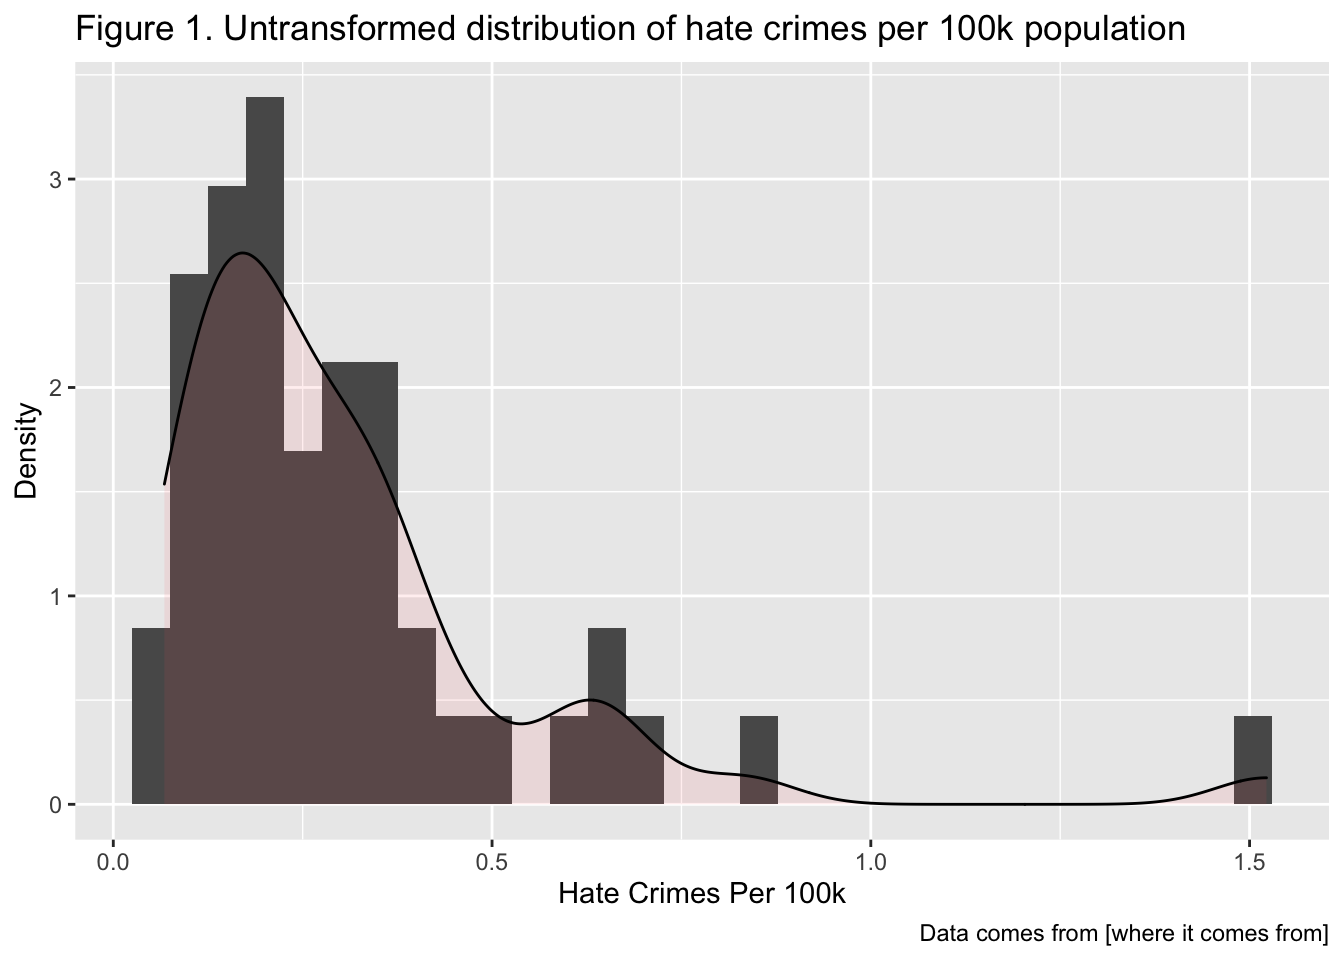
\includegraphics{project_report_files/figure-latex/unnamed-chunk-2-1.pdf}

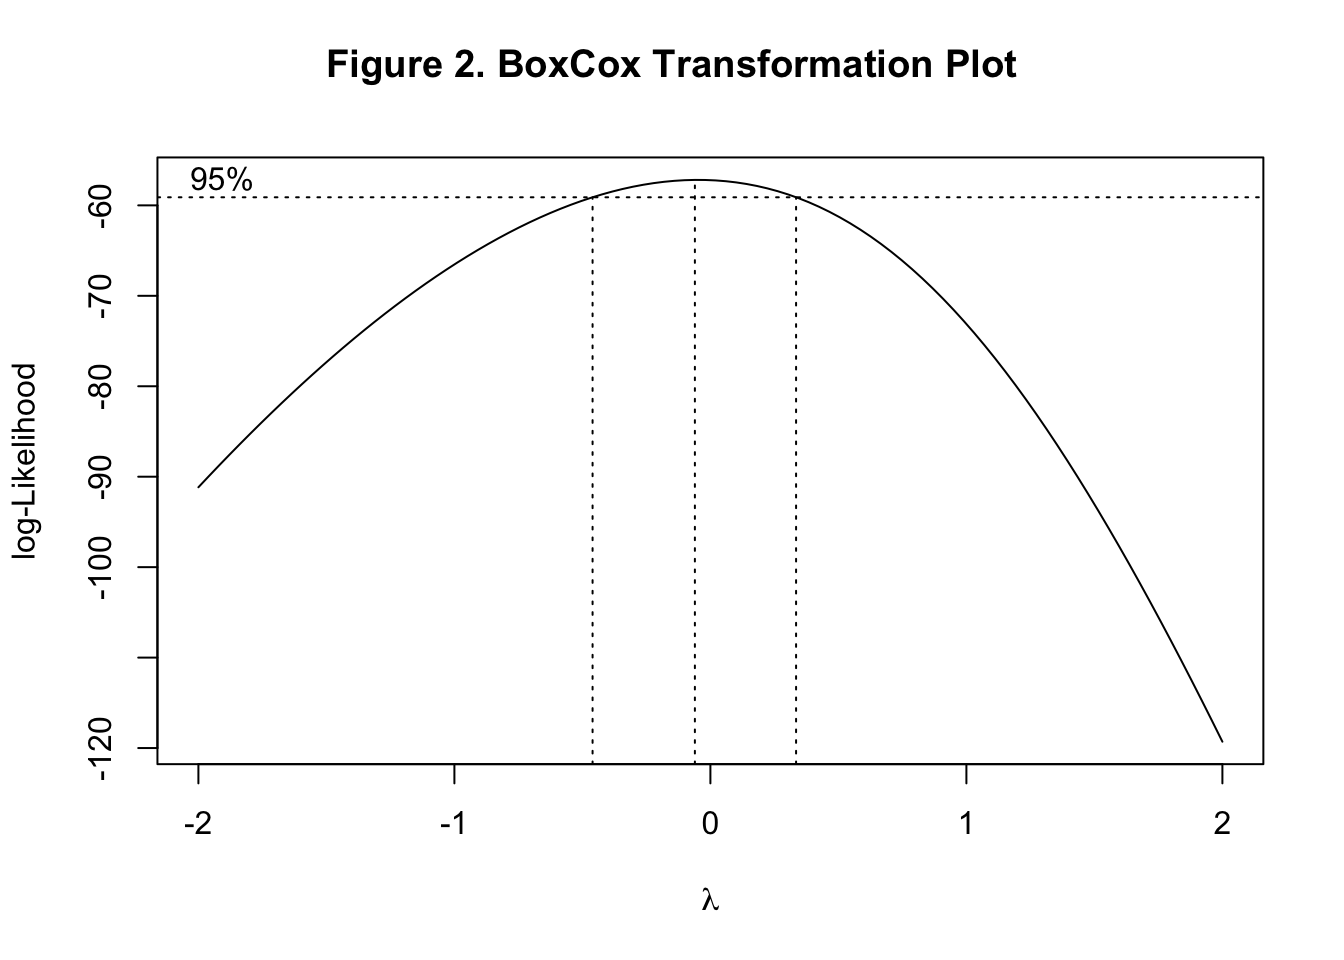
\includegraphics{project_report_files/figure-latex/unnamed-chunk-3-1.pdf}

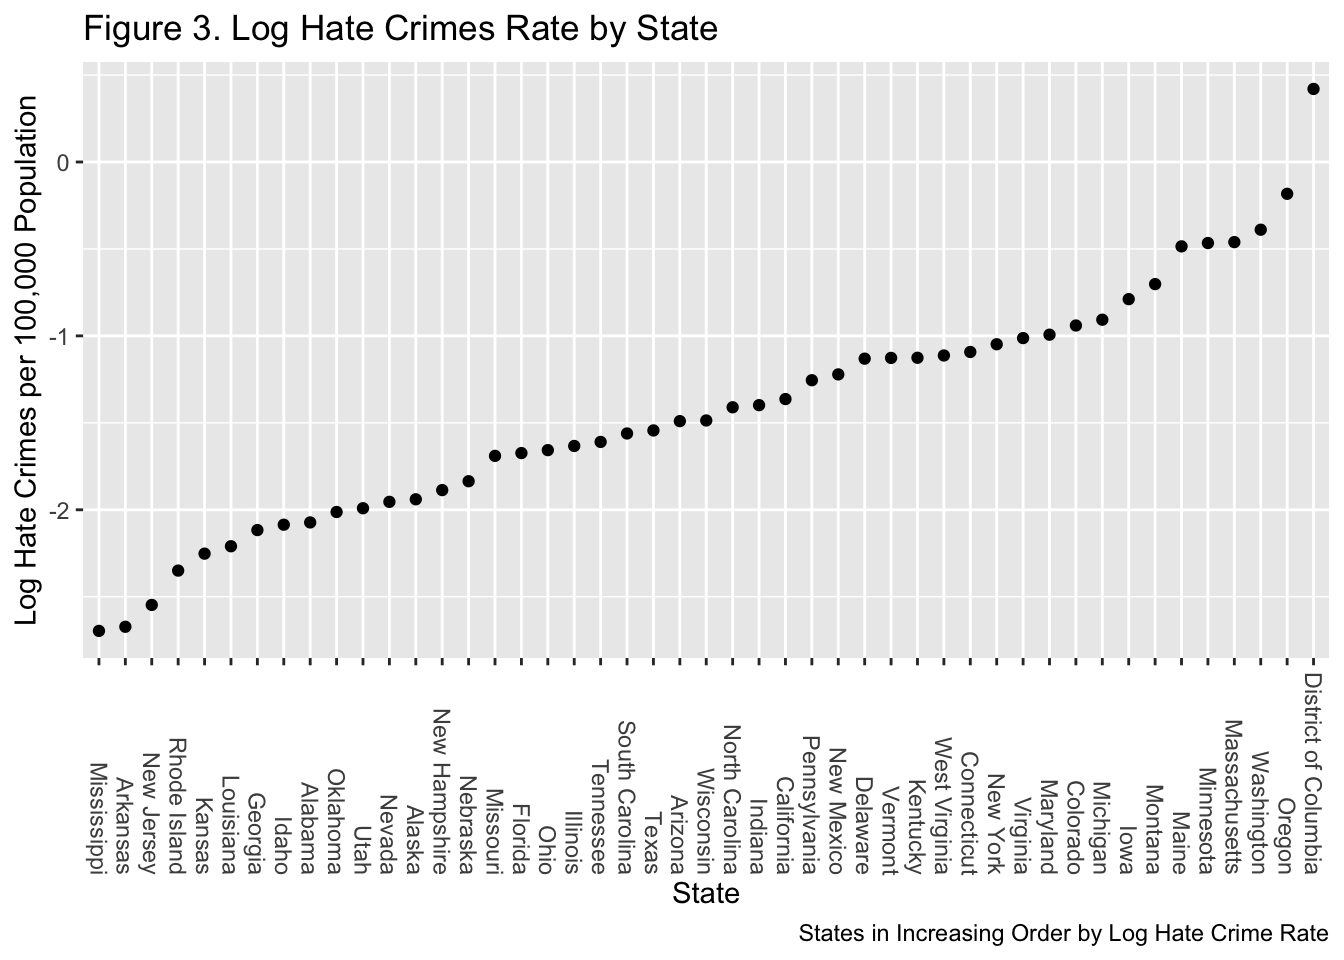
\includegraphics{project_report_files/figure-latex/unnamed-chunk-4-1.pdf}

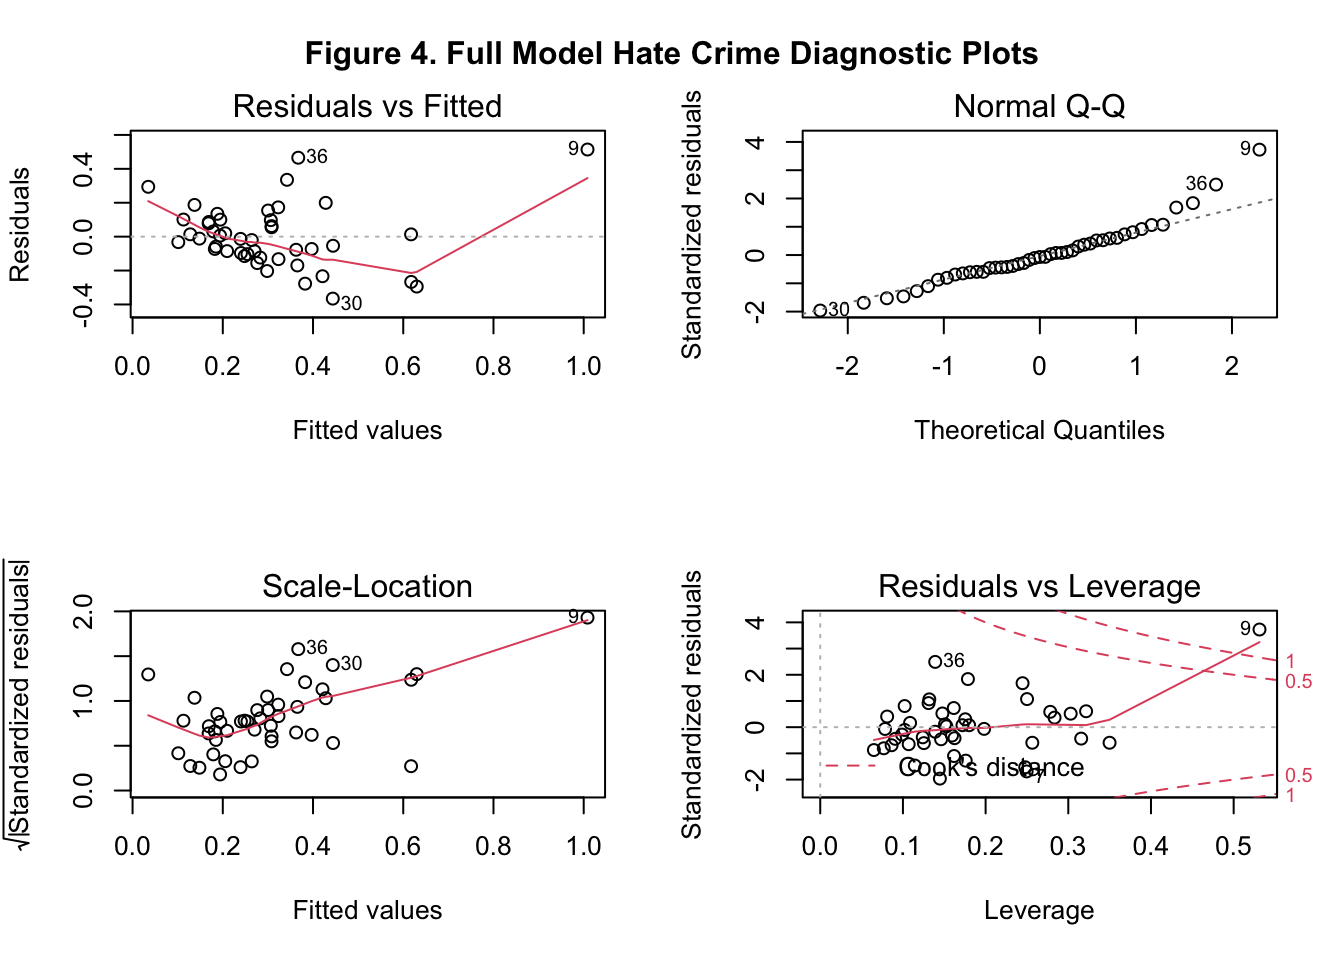
\includegraphics{project_report_files/figure-latex/unnamed-chunk-5-1.pdf}

\begin{longtable}[]{@{}ll@{}}
\caption{Table 1: Descriptive Statistics of States Reporting Hate
Crimes}\tabularnewline
\toprule
& Overall (N=47)\tabularnewline
\midrule
\endfirsthead
\toprule
& Overall (N=47)\tabularnewline
\midrule
\endhead
\textbf{Unemployment} &\tabularnewline
~~~high & 24 (51.1\%)\tabularnewline
~~~low & 23 (48.9\%)\tabularnewline
~~~Missing & 0\tabularnewline
\textbf{Urbanization} &\tabularnewline
~~~low & 23 (48.9\%)\tabularnewline
~~~high & 24 (51.1\%)\tabularnewline
~~~Missing & 0\tabularnewline
\textbf{Median Household Income} &\tabularnewline
~~~Mean (SD) & 54802.298 (9255.117)\tabularnewline
~~~Median (Q1, Q3) & 54310.000 (47629.500, 60597.500)\tabularnewline
~~~Min - Max & 35521.000 - 76165.000\tabularnewline
~~~Missing & 0\tabularnewline
\textbf{\% Adults \textgreater25yrs With HS Degree} &\tabularnewline
~~~Mean (SD) & 0.866 (0.034)\tabularnewline
~~~Median (Q1, Q3) & 0.871 (0.839, 0.895)\tabularnewline
~~~Min - Max & 0.799 - 0.915\tabularnewline
~~~Missing & 0\tabularnewline
\textbf{\% of Population Not U.S. Citizens} &\tabularnewline
~~~Mean (SD) & 0.055 (0.031)\tabularnewline
~~~Median (Q1, Q3) & 0.050 (0.030, 0.080)\tabularnewline
~~~Min - Max & 0.010 - 0.130\tabularnewline
~~~Missing & 2\tabularnewline
\textbf{Gini Index} &\tabularnewline
~~~Mean (SD) & 0.456 (0.021)\tabularnewline
~~~Median (Q1, Q3) & 0.455 (0.441, 0.468)\tabularnewline
~~~Min - Max & 0.419 - 0.532\tabularnewline
~~~Missing & 0\tabularnewline
\textbf{\% of Population Not White} &\tabularnewline
~~~Mean (SD) & 0.315 (0.150)\tabularnewline
~~~Median (Q1, Q3) & 0.300 (0.205, 0.420)\tabularnewline
~~~Min - Max & 0.060 - 0.630\tabularnewline
~~~Missing & 0\tabularnewline
\textbf{Hate Crime Rate Per 100k} &\tabularnewline
~~~Mean (SD) & 0.304 (0.253)\tabularnewline
~~~Median (Q1, Q3) & 0.226 (0.143, 0.357)\tabularnewline
~~~Min - Max & 0.067 - 1.522\tabularnewline
~~~Missing & 0\tabularnewline
\textbf{hate\_crimes\_log} &\tabularnewline
~~~Mean (SD) & -1.429 (0.676)\tabularnewline
~~~Median (Q1, Q3) & -1.486 (-1.947, -1.030)\tabularnewline
~~~Min - Max & -2.696 - 0.420\tabularnewline
~~~Missing & 0\tabularnewline
\bottomrule
\end{longtable}

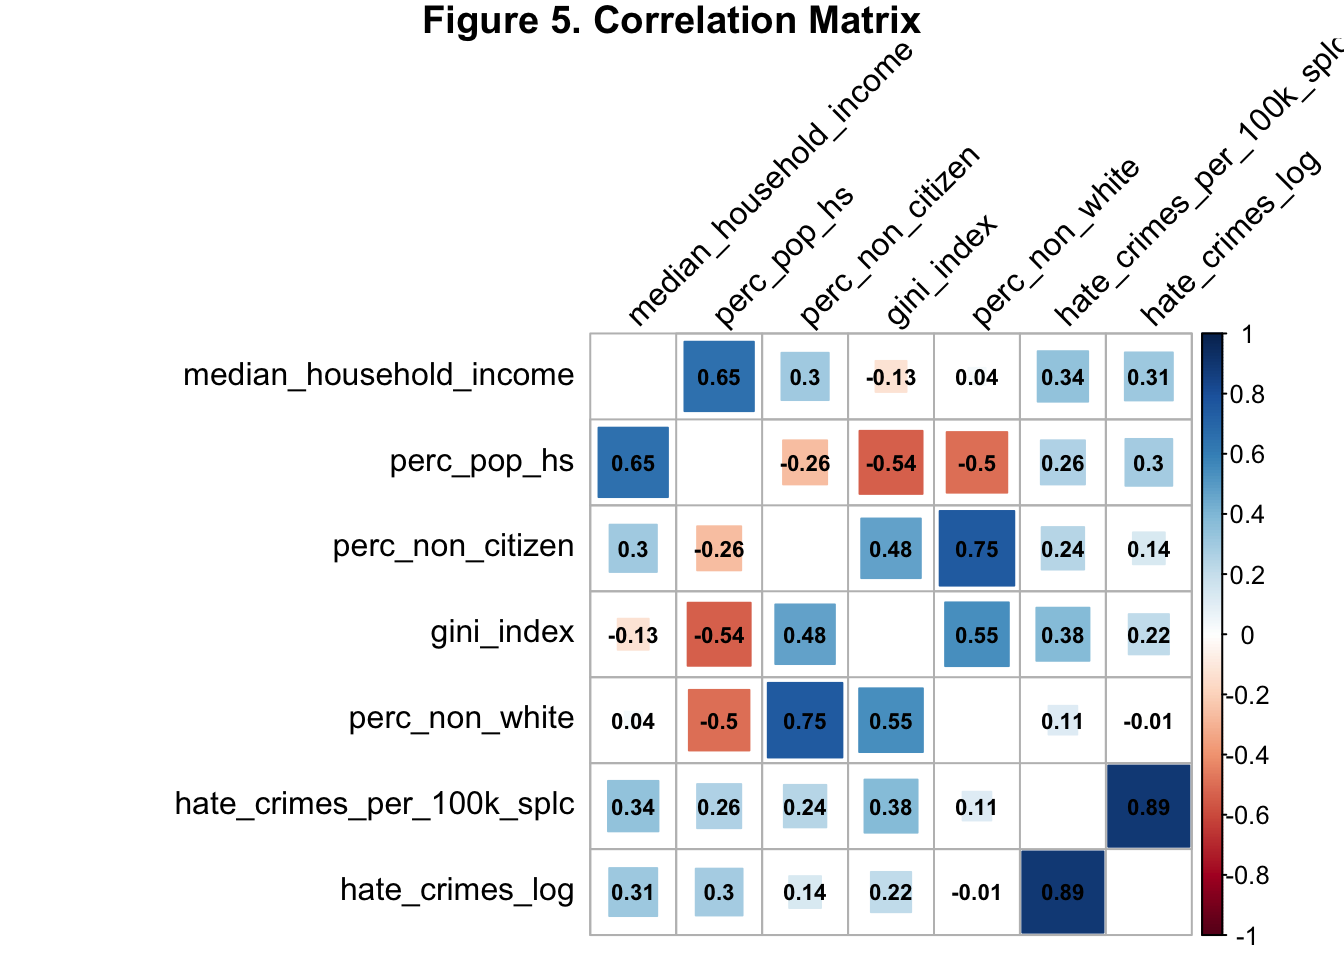
\includegraphics{project_report_files/figure-latex/unnamed-chunk-7-1.pdf}

\begin{longtable}[]{@{}lr@{}}
\toprule
& x\tabularnewline
\midrule
\endhead
unemployment & 1.426\tabularnewline
urbanization & 1.983\tabularnewline
median\_household\_income & 3.108\tabularnewline
perc\_pop\_hs & 3.895\tabularnewline
perc\_non\_citizen & 3.728\tabularnewline
gini\_index & 1.845\tabularnewline
perc\_non\_white & 3.236\tabularnewline
\bottomrule
\end{longtable}

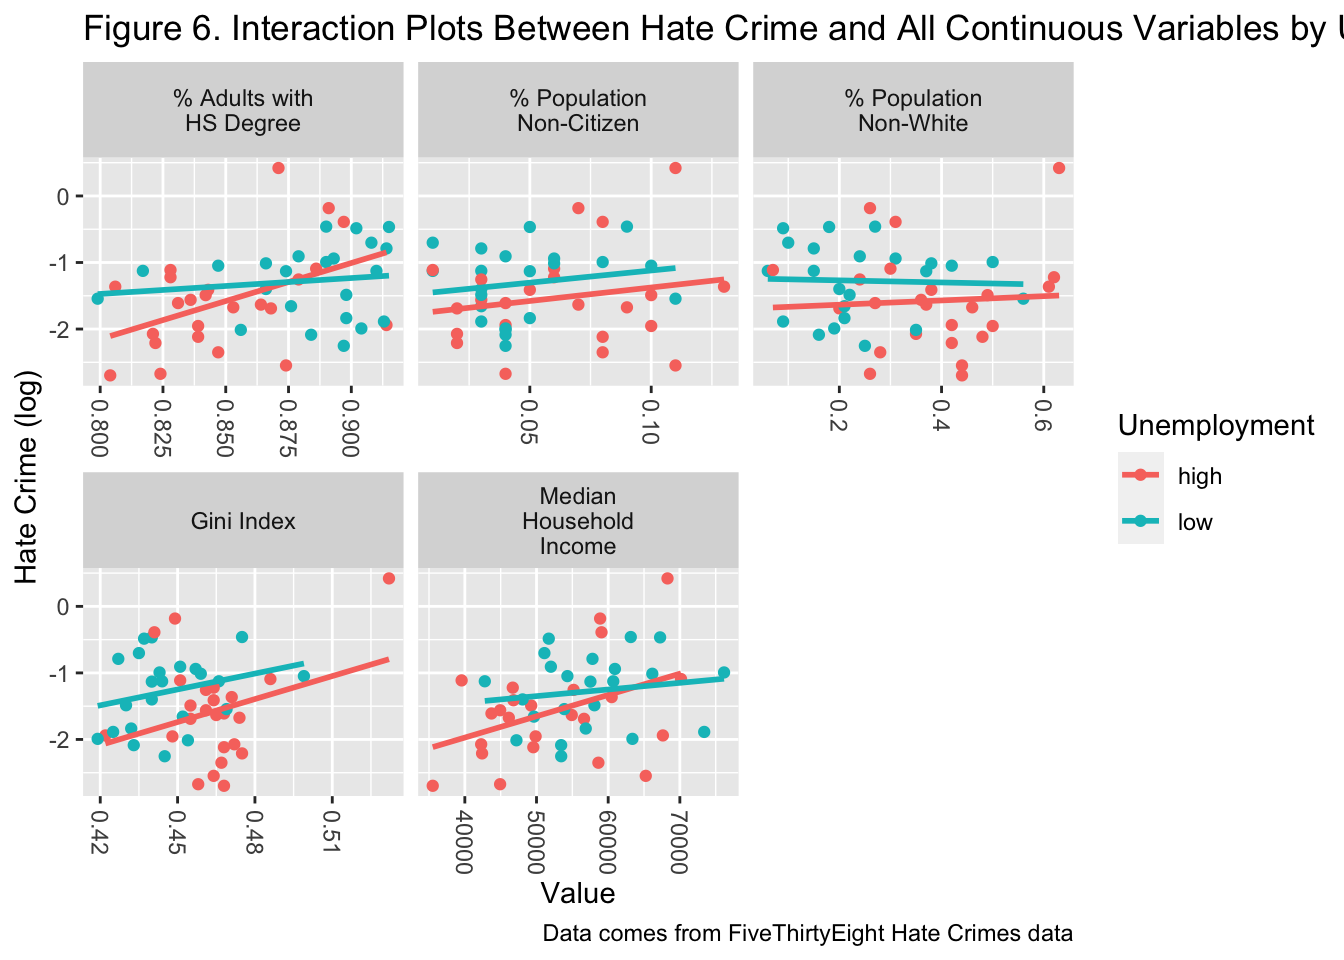
\includegraphics{project_report_files/figure-latex/unnamed-chunk-9-1.pdf}
\^{}\^{}\^{} check these plots since the numbers seem weird

{[}ADD DIAGNOSTIC PLOTS FOR DIFFERENT MODELS (2 and 3 covariate models
for both DC and not DC) (stella/vasili), ADD TABLE FOR RMSE AND ADJ R
SQUARED RESULTS (lily) AND LILY'S INTERACTION PLOTS{]}

\hypertarget{references}{%
\subsection{References}\label{references}}

(caroline)

\end{document}
